\documentclass[12pt]{report}
\usepackage[czech]{babel}
\usepackage[utf8]{inputenc}
\usepackage[IL2]{fontenc}
\usepackage{wrapfig}
\usepackage{graphicx}
\usepackage{cprotect}


\begin{document}
\setlength{\parindent}{0pt}
\begin{titlepage}

\includegraphics[scale=0.2, trim=5cm 0 0 30cm]{logo.jpg}
\begin{center}
\vspace{5cm}
{\Large
\textbf{ŘEŠENÍ KOLIZÍ FREKVENCÍ SÍTÍ VYSÍLAČÙ}
}
\end{center}
\vspace{\fill}

\begin{minipage}[t]{5cm}
\flushleft
Martin Hamet\\
os.č. A14B0254P
\end{minipage}
\hfill
\begin{minipage}[t]{7cm}
\flushright
\today
\end{minipage}
\end{titlepage}

\tableofcontents

\chapter{Zadání}
\setlength{\parskip}{\baselineskip}
Naprogramujte v ANSI C přenositelnou \textbf{konzolovou aplikaci}, která jako vstup načte z parametru příkazové řádky název textového souboru obsahující informaci o pozici vysílačů na mapě a na jeho základě přidělí každému vysílači frekvenci tak, aby jeho signál nekolidoval s vysílači v blízkém okolí.


Program se bude spouštět příkazem \texttt{freq.exe} \textit{\textless soubor-s-vysílači\textgreater}. Symbol \textit{\textless soubor-s-vysílači\textgreater} zastupuje jméno textového souboru, který obsahuje informaci o rozmístění vysílačů na mapě a o dostupných vysílacích frekvencí, které jim je možné přidělit.


Váš program tedy může být během testování spuštěn například takto:\\
\texttt{freq.exe vysilace-25.txt}


Výsledkem práce programu bude výpis do konzole se seznamem přidělených frekvencí každému vysílači ze vstupního souboru (viz Specifikace výstupu programu). V případě chyby nebo neřešitelné situace skončí program výpisem příslušné chybové hlášky.


Pokud nebude na příkazové řádce uveden právě jeden argument, vypíše chybové hlášení a stručný návod k použití programu v angličtině podle běžných zvyklostí (viz např. ukázková semestrální práce na webu předmětu Programování v jazyce C). \textbf{Vstupem programu je pouze argument na příkazové řádce -- interakce s uživatelem pomocí klávesnice či myši v průběhu práce programu se neočekává.}


Hotovou práci odevzdávejte v jediném archivu typu \textbf{ZIP} prostřednictvím automatického odevzdávacího a validačního systému. Postupujte podle instrukcí uvedených na webu předmětu. Archiv nechť obsahuje všechny zdrojové soubory potřebné k přeložení programu, \textbf{makefile} pro Windows i Linux (pro překlad v Linuxu připravte soubor pojmenovaný \texttt{makefile} a pro Windows \texttt{makefile.win}) a dokumentaci ve formátu \textbf{PDF} vytvořenou v typografickém systému \TeX, resp. \LaTeX. Bude-li některá z částí chybět, kontrolní script Vaši práci odmítne.


Podrobnější informace o vstupu a výstupu programu jsou uvedeny v souboru \textbf{zadani.pdf}.

\chapter{Analýza úlohy}
Vstupem programu budou dostupné frekvence a rozmístění vysílačů na dvourozměrné mapě. Úkolem je přiřadit vysílačům frekvence, tak aby nedocházelo ke kolizi signálů. Každý vysílač pokryje oblast danou dosahem svého signálu a k rušení signálu dochází v případě že dva, nebo více různých vysílačů se stejnou frekvencí pokrývá stejnou část území. Taková situace nesmí nastat. Volných frekvencí máme ovšem omezený počet. Budeme se tedy snažit využít co nejmenší počet z těchto dostupných frekvencí.

Nejprve je nutné zjistit, které vysílače navzájem kolidují. Vysílačům bez kolizí snadno přiřadíme první dostupnou frekvenci. Pro hledání kolizních vysílačů bude nejsnazší zjistit vzdálenost každých dvou vysílačů a pokud jejich vzdálenost bude menší než součet dosahů jejich signálů označíme je za kolizní.

\begin{wrapfigure}[9]{l}{5cm}
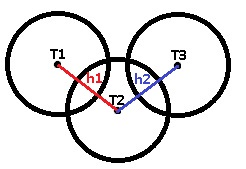
\includegraphics[width=5cm]{img1.jpg}
\caption{Kolize třech vysílačů.}
\label{obr1}
\end{wrapfigure}

Kolizním vysílačům by bylo možné přiřazovat stále vyšší frekvence, ale tím bychom použili příliš mnoho dostupných frekvencí. Například podle obr. \ref{obr1}. Vysílač T1 koliduje pouze s T2 a proto T3 může mít stejnou frekvenci jako T1. Pro usnadnění práce si vytvoříme graf kolizí, kde vrcholy grafu jsou jednotlivé vysílače a hrany mezi vysílači představují kolizi (hrany h1 a h2 v obr. \ref{obr1}). 


Převedením problému do grafu získáme souvislé komponenty grafu, kde dochází ke kolizím. Stačí tedy vyřešit přidělování frekvencí v každé komponentě zvlášť.

\section{Graf kolizí} \label{graf_kolizi}
Neorientovaný graf kolizí se skládá z vrcholů které reprezentují vysílače. Hranou jsou propojené pouze vrcholy, které jsou natolik blízko u sebe že může docházet ke kolizi signálů. Protože mají všechny vysílače stejný dosah signálu zjišťujeme pouze zda jsou vrcholy od sebe vzdálené méně než dvojnásobek dosahu signálu. Vytvoření grafu kolizí z mapy vysílačů je znázorněno na obr. \ref{obr2}.

\begin{figure}[h]
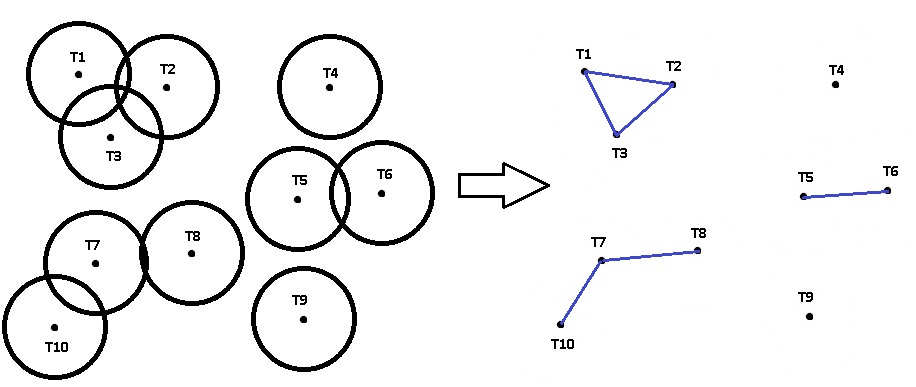
\includegraphics[width=13cm]{img2.jpg}
\caption{Vysílače a dosah jejich signálů (vlevo) a výsledný kolizní graf (vpravo).
\label{obr2}}
\end{figure}

\pagebreak
\section{Přiřazování frekvencí} \label{prirazovani_frekvenci}
\begin{enumerate}
\item Vytvoříme graf kolizí (viz výše).
\item Označíme frekvence všech vrcholů za nepřiřazené.
\item Pokud ještě existuje nějaký vrchol s nepřiřazenou frekvencí.Procházíme všechny vrcholy grafu a vybereme vrchol s nepřiřazenou frekvencí. Pokud takový vrchol neexistuje ukončíme algoritmus, protože bylo nalezeno řešení.
\item Vybranému vrcholu postupně přiřazujeme dostupné frekvence od nejnižší dokud nenalezneme takovou, že z vrcholu nevede hrana k vrcholu se stejnou frekvencí. Pokud nemáme dostatečný počet dostupných frekvencí ukončíme algoritmus, protože se nepodařilo nalézt řešení.
\item Pokračujeme od bodu 3.
\end{enumerate}

Tento algoritmus funguje ovšem v některých situacích nevhodné pořadí vrcholů při jejich průchodu snadno ukončí algoritmus s nenalezením řešení. Podle obr. \ref{obr3} kde máme pouze dvě dostupné frekvence a pořadí ve kterém procházíme vrcholy grafu je T1, T2, T3, T4.

\begin{wrapfigure}[11]{l}{7cm}
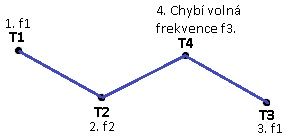
\includegraphics[width=7cm]{img3.jpg}
\caption{Přiřazování frekvencí.}
\label{obr3}
\end{wrapfigure}

Jak je vidět na obrázku vrcholu T4 byla přiřazována frekvence jako poslední. Tohoto problému s pořadím v vrcholů, pokud jsou v jedné souvislé komponentě grafu, se můžeme částečně zbavit budeme-li graf procházet nejprve po nalezených sousedech až poté budeme hledat další vrchol s nepřiřazenou frekvencí v seznamu všech vrcholů. Takový průchod můžeme zajistit např. frontou, nebo zásobníkem do kterého budeme ukládat nalezené vrcholy. Budeme muset tedy upravit bod 4. kde je potřeba ještě projít všechny sousedy vybraného vrcholu a pokud nemají přiřazenou frekvenci přidat je do zásobníku pokud v něm nejsou.

Fronta by zajistila průchod z vybraného vrcholu do šířky (tzv. BFS). Jak je naznačeno na obr. \ref{obr4}. Počáteční vrchol byl vrchol 1. a byla mu přidělena první frekvence f1. Průchod do šířky nejprve projde všechny sousedy počátečního vrcholu, dále sousedy sousedů atd. Oproti zásobníku, který zajistí průchod do hloubky (tzv. DFS). Naznačeno na obr. \ref{obr5}. 

Průchod do hloubky se nejprve snaží co nejvíce zanořit do grafu, přes ještě neobjevené vrcholy. Vznikne tedy nejprve kostra spojité komponenty, jak je naznačeno červenou čarou na obr. \ref{obr5}, na které se střídají první dvě dostupné frekvence. V obou případech BFS i DFS je výsledek závislý na pořadí uložených sousedů u vrcholu a celkově se nedá říci, který ze zmíněných způsobů bude výhodnější. V každém případě oba dokážou vždy vyřešit komponenty, nebo jejich částí, řetězového typu, jako byla komponenta na obr. \ref{obr3}. Do řešení jsem ve výsledku zvolil způsob se zásobníkem kvůli nepatrně snazší implementaci, protože oba způsoby vypadají ekvivalentní co se týče nalezení řešení.

\begin{figure}[ht]
\begin{minipage}{6cm}
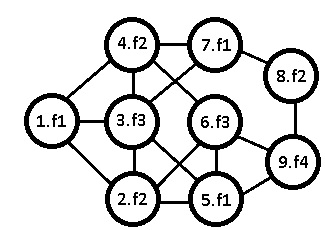
\includegraphics[width=6cm]{img4.jpg}
\caption{BFS}
\label{obr4}
\end{minipage}
\hspace{\fill}
\begin{minipage}{6cm}
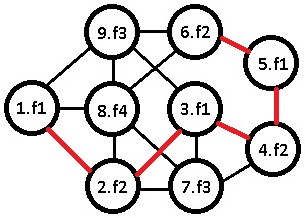
\includegraphics[width=6cm]{img5.jpg}
\caption{DFS}
\label{obr5}
\end{minipage}
\end{figure}

Tento způsob by řešil problém po souvislých komponentách jak bylo řečeno výše. Ovšem není zajištěno že algoritmus vždy nalezne řešení. Při nevhodném pořadí přiřazení sousedů a nedostatku frekvencí tento způsob nemusí fungovat, i když řešení existuje. Tento problém se nedá s jistotou vyřešit. S vyšším počtem dostupných frekvencí a s menším počtem kolizních vysílačů roste šance úspěšného nalezení řešení.

\section{Datové struktury}
\subsection{Dostupné frekvence}
Dostupné frekvence se budou načítat ze vstupního souboru (viz kapitola \ref{format_vst_souboru}) bez předem známého počtu. Každá frekvence má svoje id a vlastní hodnotu frekvence v [Hz]. Tím se nabízí dvě možnosti. Vytvoření klíčovací tabulky pro id a ve vlastním programu pracovat pouze s id dané frekvence a pro výsledek rozklíčovat jednotlivé id podle tabulky, nebo vytvoření struktury pro každou frekvenci, která by obsahovala svoje id a frekvenci. Z pohledu paměťové náročnosti jsou obě možnosti ekvivalentní, proto jsem zvolil možnost se strukturou. V případě nutnosti úprav programu nebo dodatečného počítání s vlastní hodnotou bude snazší program rozšířit.

Vzhledem k tomu že se snažíme použít co nejmenší počet dostupných frekvencí budeme seznam frekvencí procházet vždy od začátku. Nepředpokládají se žádné náhodné přístupy doprostřed tohoto seznamu a také dopředu neznáme jejich počet ve vstupním souboru, proto se přikláním k vytvoření spojového seznamu frekvencí místo uložení do pole.

\subsection{Vysílače}
Vysílače načítáme ze vstupního souboru podobně jako dostupné frekvence, každý vysílač bude mít vlastní identifikační číslo a souřadnice (x,y) určující umístění na dvourozměrné mapě. Tentokrát bude potřeba jednotlivým vysílačům přiřazovat frekvence a jejich sousedy v případě grafu kolizí. Struktura je tedy výhodnou volbou.

Budeme se snažit udržet vyřešení problému ve dvou průchodech všech vysílačů, po načtení vstupních dat. Prvním průchod bude nutný pro vytvoření grafu kolizí (viz \ref{graf_kolizi}). Ve druhém průchodu budeme už přiřazovat frekvence jednotlivým vysílačům (viz \ref{prirazovani_frekvenci}). 

Sousedé každého vysílače by měli být reprezentováni jednosměrným spojovým seznamem vzhledem k tomu že nevíme jak hustý graf kolizí vznikne a tím kolik bude mít každý vysílač sousedů. Je zde další možnost použití id jednotlivých vysílačů a v seznamu sousedů mít pouze id daných vysílačů. Tuto možnost jsem (ze stejných důvodů jako u frekvencí) zavrhnul a sousedé budou tvořeni ukazateli přímo na struktury daných vysílačů. Díky této volbě by neměl být nutný náhodný přístup doprostřed seznamu vysílačů a můžeme také použít jednosměrný spojový seznam. Tím se opět zjednodušuje načítání neznámého počtu vysílačů ze vstupního souboru vůči použití pole.

\subsection{Zásobník}
U zásobníku se nabízí reprezentace polem. Po vytvoření grafu kolizí  by jsme měli vědět kolik by měla být maximální velikost zásobníku. V zásobníku by se mohli najednou vyskytovat všechny kolizní vysílače najednou. Taková možnost je sice nepravděpodobná, ale možná např. pro malý počet vstupních vysílačů blízko sebe. Bylo by nutné vytvořit dynamicky se zvětšující zásobník. 

\begin{wrapfigure}[9]{r}{6cm}
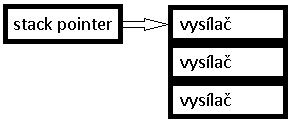
\includegraphics[width=6cm]{img7.jpg}
\caption{Zásobník polem.}
\label{obr6}
\end{wrapfigure} 
Z pohledu paměťové náročnosti a za předpokladu že by jsme měli dostatečnou velikost zásobníku, je výhodnější reprezentace polem, která pro ukládání vysílačů (bez vlastní režie zásobníku) potřebuje uložit jeden ukazatel na jeden vysílač (viz obr. \ref{obr6}). Naproti tomu zásobník reprezentovaný spojovým seznamem potřebuje ukazatele dva (jeden pro vlastní vysílač a druhý pro další položku spojového seznamu) jak se znázorněno na obr. \ref{obr7}. Tedy pro velmi hustý graf by se vyplatil zásobník polem, ovšem by se muselo ošetřit dynamické zvětšování pro krajní případy a ne všechna alokovaná paměť by se nutně využívala. 

\pagebreak
\begin{wrapfigure}[10]{l}{7cm}
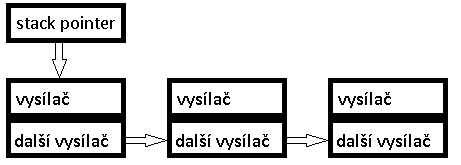
\includegraphics[width=7cm]{img6.jpg}
\caption{Zásobník spojovým seznamem.}
\label{obr7}
\end{wrapfigure}

Výhoda použití spojového seznamu spočívá v jeho dynamické velikosti z podstaty spojového seznamu. S předpokladem že graf bude spíše řídký a případ, že každý vysílač koliduje s každým nebude běžně nastávat, budu realizovat zásobník spojovým seznamem. V našem problému ovšem nebudeme potřebovat zásobník pro jiné prvky než vysílače. Použijeme tedy struktur, které budou potřeba pro spojový seznam všech vysílačů. Zásobník zůstane použitelný pouze pro vysílače a implementace bude jednodušší.

\chapter{Popis implementace}
\subsection{Popis datových struktur}
\subsubsection{Dostupné frekvence}
Struktura \texttt{frequency} --- Představuje dostupnou frekvenci. Obsahuje id a vlastní hodnotu frekvence v [Hz] a v programu se pracuje s frekvencí výhradně uložené v této struktuře.

Struktura \texttt{frequencies} --- obsahuje ukazatel na strukturu \texttt{frequency} a ukazatel na další \texttt{frequencies}. Tato struktura slouží pro vytváření spojového seznamu z dostupných frekvencí. Pokud je to poslední frekvence v seznamu je její ukazatel na další \texttt{frequencies} nastaven na \texttt{NULL}.

\subsubsection{Vysílače}
Struktura \texttt{coordinates} --- Obsahuje pouze informace o souřadnicích. Přiřazuje se danému vysílači jako reprezentace jeho pozice na mapě.
\pagebreak
Struktura \texttt{transmitter} --- Představuje vysílač. Obsahuje id vysílače,  informaci o jeho pozici strukturou \texttt{coordinates}, ukazatel na přiřazenou frekvenci \\ \texttt{frequency} a odkaz na první prvek spojového seznamu sousedů \texttt{neighbours}. Pokud vysílač nemá zatím přiřazenou žádnou frekvenci je ukazatel nastaven na \texttt{NULL}, to samé platí pro sousedy.

Struktura  \texttt{neighbours} --- Slouží k vytvoření spojového seznamu vysílačů stejně jako \texttt{transmitters}, v tomto případě představuje seznam sousedů který se přiřadí jednomu vysílači. Obsahuje odkaz na vysílač \texttt{transmitter} (který je sousedem) a odkaz na dalšího souseda \texttt{neighbours}. Ukazatel na dalšího souseda je nastaven na \texttt{NULL} pokud je to poslední soused.

Struktura  \texttt{transmitters} --- Slouží k vytvoření spojového seznamu vysílačů. Obsahuje ukazatel na vysílač \texttt{transmitter} a odkaz na další prvek seznamu \texttt{transmitters}. Pokud je to poslední prvek je odkaz na další nastaven na \texttt{NULL}.

\subsection{Moduly}
\setlength{\parskip}{1pt}

\subsubsection{\Large{\texttt{freq.c}}}
Jedná se o hlavní modul, který se stará o načítání vstupního souboru, volání funkčního modulu \verb|function.c| a uvolnění všech alokovaných prostředků (i v případě nenalezení řešení), které byly potřeba pro ostatní moduly.

\cprotect\paragraph{Ukazatel \verb|freqs_head|}
je ukazatel na hlavičku seznamu všech dostupných frekvencí.

\cprotect\paragraph{Ukazatel \verb|trans_head|}
je ukazatel na hlavičku seznamu všech vysílačů.

\cprotect\paragraph{Ukazatel \verb|m_stack|}
je ukazatel na vrchol zásobníku pro vysílače.

\cprotect\paragraph{Hodnota \verb|input_buffer_size|}
je maximální délka jednoho řádku ve vstupním souboru.

\cprotect\paragraph{Funkce \verb|load_available_frequencies|}
zistí zda se na začátku souboru nachází korektně pojmenovaná sekce dostupných frekvencí. Pokud ne vypíše do konzole chybu a vrátí hodnotu \texttt{1}. Pokud byla rozpoznána sekce dostupných frekvencí načítá frekvence pomocí funkce \verb|read_frequency|. Dokud tato funkce úspěšně načítá řádky frekvence sou přidávány do seznamu dostupných frekvencí funkcí \verb|frequencies_add_frequency| z modulu \texttt{function.c}. Po úspěšném načtení celého bloku frekvencí funkce vrátí hodnotu \texttt{0}.

\cprotect\paragraph{Funkce \verb|load_radius|}
zistí zda se na dalším řádku souboru nachází korektně pojmenovaná sekce dosahu signálu vysílačů. Pokud ne vypíše do konzole chybu a vrátí hodnotu \texttt{2}. Pokud byla rozpoznána sekce dosahu signálu vysílačů načte hodnotu a pomocí funkce \verb|transmitters_set_radius| z modulu \texttt{transmitters.c} ji uloží. Po úspěšném načtení hodnoty přejde k dalšímu řádku souboru a vrátí hodnotu \texttt{0}.

\cprotect\paragraph{Funkce \verb|load_transmitters|}
zjistí zda se na začátku souboru nachází korektně pojmenovaná sekce vysílačů. Pokud ne vypíše do konzole chybu a vrátí hodnotu \texttt{3}. Pokud byla rozpoznána sekce vysílačů načítá frekvence pomocí funkce \verb|read_transmitter|. Dokud tato funkce úspěšně načítá řádky vysílačů sou přidávány do seznamu všech vysílačů funkcí \\  \verb|transmitters_add_transmitter| z modulu \texttt{transmitters.c}. Po úspěšném načtení celého bloku vysílačů funkce vrátí hodnotu \texttt{0}.

\cprotect\paragraph{Funkce \verb|load_file|}
se postará o načtení vstupního souboru pomocí funkcí:\\
\verb|load_available_frequencies|\\
\verb|load_radius|\\
\verb|load_transmitters|.

\cprotect\paragraph{Funkce \verb|main|}
zajistí inicializaci hlaviček, zkontroluje počet argumentů a pokusí se načíst vstupní soubor funkcí \verb|load_file|. Při úspěšném načtení souboru zajistí vytvoření kolizního grafu voláním funkce \\ \verb|function_find_collisions| a následně přiřazení frekvencí vysílačům funkcí \verb|function_assing_frequencies|. Při úspěšném přiřazení vypíše všechny vysílače do konzole a uvolní alokovanou paměť funkcí \texttt{clear}. Pokud program nedokázal najít řešení nebo nastala jiná chyba, vypíše příslušnou chybovou hlášku do konzole a uvolní paměť voláním \texttt{clear}.

\subsubsection{\Large{\texttt{frequencies.c}}}
Modul obsahuje funkce pro snadné vytvoření a smazání spojového seznamu dostupných frekvencí.

\cprotect\paragraph{Funkce \verb|frequencies_add_frequency|}
vytvoří novou frekvenci \texttt{frequency} podle předaných parametrů a zařadí ji do seznamu dostupných frekvencí předaného v podobě ukazatele na poslední přidaný prvek. Po zařazní nové frekvence vrátí ukazatel na poslední zařazený prvek. Pokud se jedná o první prvek seznamu stačí místo posledního prvku do funkce předat ukazatel \texttt{NULL}.

Dále modul obsahuje funkce pro výpis frekvence, nebo frekvencí do konzole. Na funkci celého programu nemají vliv. Jsou určeny k testování.

\subsubsection{\Large{\texttt{transmitters.c}}}
Modul obsahuje funkce pro vytvoření seznamu vysílačů, přidávání jejich sousedů, mazání spojového seznamu vysílačů a výpis seznamu do konzole. Tento modul je závislý na modulu \texttt{frequencies.c}, protože jeden z atributů vysílače je jeho frekvence.

\cprotect\paragraph{Funkce \verb|transmitters_add_transmitter|}
vytvoří nový vysílač podle předaných parametrů a zařadí ho do seznamu vysílačů předaného pomocí ukazatele na poslední přidaný prvek. Po zařazení nového vysílače vrátí ukazatel na poslední zařazený prvek. Pokud se jedná o první prvek seznamu stačí místo posledního prvku do funkce předat ukazatel \texttt{NULL}.

\cprotect\paragraph{Funkce \verb|transmitters_print_all|}
vypíše do konzole předaný prvek spojového seznamu a všechny následující. Tato funkce je použita jako standardní výstup programu a je volána až po úspěšném přiřazení frekvencí všem vysílačům.

Dále modul obsahuje funkce pro výpis jednoho vysílače nebo sousedů konkrétního vysílače do konzole. Jsou určeny k testování.
\pagebreak
\cprotect\subsubsection{\Large{\verb|transmitters_stack.c|}}
Modul slouží pro vytvoření a obsluhu zásobníku. Do zásobníku lze vkládat pouze vysílače \texttt{transmitter}. Modul je tedy závislý na modulu \\ \texttt{transmitters.c}.

\cprotect\paragraph{Funkce \verb|t_stack_pop|}
vyjme prvek ze zásobníku, předaného jako ukazatel na ukazatele vrcholu zásobníku, a ukazatel na něj vloží do předaného ukazatele na ukazatele \texttt{transmitter}. Dále uvolní alokovanou paměť kterou zásobník potřeboval. Pokud tedy odebereme všechny prvky ze zásobníku není nutné volat funkci \verb|t_stack_free_stack|.

\subsubsection{\Large{\texttt{function.c}}}
Modul je závislý na všech předchozích, protože poskytuje funkce pro nalezení kolizí vysílačů, přiřazování frekvencí atp.

\cprotect\paragraph{Hodnota \verb|power_radius|}
je umocněný dosah signálu vysílačů. Mocnina je zde kvůli snažšímu porovnávání vzdáleností dvou vysílačů, aby nebylo nutné pokaždé vzdálenost odmocňovat.

\cprotect\paragraph{Ukazatel \verb|f_encountered|}
je ukazatel na ukazatel na \texttt{NULL}. Používá se pouze jako označení vysílače za nalezený bez přiřazené frekvence, který se přidává do zásobníku. Tímto označením snadno zabráníme zbytečnému přidání některého vysílače do zásobníku dvakrát. Tento ukazatel se vytváří při volání funkce \verb|function_assing_frequencies|.

\cprotect\paragraph{Funkce \verb|function_find_collisions|}
očekává předání hlavičky spojového seznamu vysílačů. Prochází všechny dvojice vysílačů a zjišťuje zda může nastat kolize signálu pomocí funkce \verb|calculate_collision|. Pokud je nalezena kolize dvou vysílačů, je mezi nimi vytvořena neorientovaná hrana pomocí seznamů sousedů. Díky tomu že vytváříme neorientované hrany, hlavní cyklus prochází seznam vysílačů pouze jednou a sekundární cyklus prochází pouze zbývající vysílače. Nekontroluje se tedy nikdy dvakrát stejná dvojice, což znamená urychlení v případě velkého počtu vysílačů. Tato funkce se volá z hlavního modulu \verb|freq.c| po načtení vstupních dat.

\cprotect\paragraph{Funkce \verb|is_possible_to_assign|}
očekává předání vysílače, kterému byla dočasně přiřazena frekvence a zjišťuje zda vysílač má nějaké sousedy, pokud nemá funkce úspěšně skončí a vysílači zůstane frekvence přiřazená. V případě že má sousedy postupně je prochází a zjišťuje zda frekvence předaného vysílače nekoliduje. Všechny jeho sousedy, kteří nemají přiřazenou frekvenci a ještě nejsou v zásobníku označí \verb|f_encountered| za nalezené a vloží je do zásobníku. Pokud nenastala žádná kolize se sousedem funkce úspěšně skončí a vrací hodnotu \texttt{0}. Pokud dojde ke kolizi vrací hodnotu \texttt{1}. Volá se pouze vnitřně z tohoto modulu.

\cprotect\paragraph{Funkce \verb|assign_frequency|\label{fassign_frequency}}
očekává předání vysílače a hlavičky seznamu dostupných frekvencí. Funkce přiřazuje vysílači frekvence ze seznamu a testuje úspěšné přiřazení funkcí \verb|is_possible_to_assign|. Pokud přiřazení neproběhne a vyčerpá se seznam dostupných frekvencí funkce vrátí \texttt{1}. Při úspěšném přiřazení vrací \texttt{0}. Volá se pouze vnitřně z tohoto modulu.

\cprotect\paragraph{Funkce \verb|function_assing_frequencies|}
očekává ukazatel na hlavičku seznamu všech vysílačů, ukazatel na hlavičku všech dostupných frekvencí a ukazatel na ukazatel prázdného zásobníku. Funkce prochází seznam všech vysílačů. Vysílač který nemá přiřazenou frekvenci vloží do zásobníku a čeká na konec vedlejšího cyklu. Tento cylus vybírá vysílače ze zásobníku a pokouší se jim přiřazovat frekvence pomocí funkce \verb|assign_frequency|. Tato funkce přidává do zásobníku další vysílače (viz \ref{fassign_frequency} Funkce \verb|assign_frequency|). Vedlejší cyklus tedy končí v případě, že byly úspěšně přiřazeny frekvence celé souvislé komponentě ve které se daný vysílač nacházel. Pokud se přiřazení některému z vysílačů nepodařilo funkce končí a vrací hodnotu \texttt{1}. Při úspěšném přiřazení všem vysílačům vrací \texttt{0}. Tato funkce se volá z hlavního modulu \verb|freq.c| po načtení vstupních dat a vytvoření sousedů pomocí funkce \verb|function_find_collisions|.

\chapter{Uživatelská příručka}
\setlength{\parskip}{\baselineskip}
\section{Program}
\subsection{Přeložení programu}
\subsubsection{UNIX/Linux}
Správnou kompilaci programu lze zajistit použitím příkazu \texttt{make} v adresáři se zdrojovými soubory a se souborem makefile.

\subsubsection{Win32/64}
Správnou kompilaci programu lze zajistit použitím příkazu:  \texttt{mingw32-make} 
\\v adresáři se zdrojovými soubory a se souborem \texttt{makefile}. Pro tento způsob je nutné mít nainstalovaný balík \texttt{mingw32} a překladač \texttt{gcc} a oba přidané v sytémové proměnné \texttt{PATH}.

\subsection{Další funkce makefile}
Vytvořené soubory \texttt{makefile} a \texttt{makefile.win} obsahují další funkčnost pro usnadnění práce se zdrojovými kódy přidáním klíčového slova za příkaz \texttt{make}.

\textbf{Klíčová slova:}\\
\texttt{clean} --- smaže všechny objektové soubory v adresáři včetně \texttt{freq.exe}.

\texttt{rebuild} --- smaže všechny objektové soubory v adresáři včetně \texttt{freq.exe} a provede znovu kompletní kompilaci.

\subsection{Spuštění programu}
Program se spouští z příkazové řádky příkazem: \\
\texttt{freq.exe} \textit{\textless soubor-s-vysílači.txt\textgreater}\\
Jediný a povinný parametr je název vstupního textového souboru. Který se nachází ve stejném adresáři jako \texttt{freq.exe}.
Příkaz na spuštění programu by mohl například vypadat jako na obr. \ref{obr8}.

\begin{figure}[h]
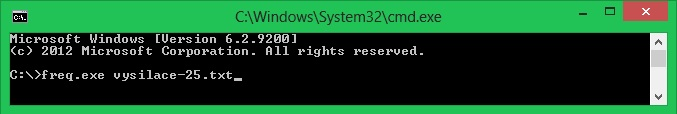
\includegraphics[width=13.7cm]{img8.jpg}
\caption{Spuštění programu.}
\label{obr8}
\end{figure}

Při úspěšném nalezení šeření program vypíše do konzole všechny vysílače reprezentované jejich vlastním \texttt{ID} a přiřazenou hodnotou frekvence v Hertzích.

\section{Formát vstupního souboru}\label{format_vst_souboru}
Vstupní textový soubor začíná řetězcem \texttt{Available frequencies:} za kterým následují dostupné frekvence. Na každém řádku je pouze jedna frekvence ve formátu: \texttt{ID-frekvence hodnota}\\
kde \texttt{ID-frekvence} je identifikační (celé kladné) číslo a frekvence jsou v souboru seřazeny vzestupně podle jejich ID. Hodnota frekvence \texttt{hodnota} je udaná v Hertzích.

Dále následuje na samostatném řádku řetězec \texttt{Transmission radius:} za kterým je udán dosah signálu všech vysílačů udaný jako celé kladné číslo.

Na dalším řádku následuje řetězec \texttt{Transmitters:} za kterým následují vysílače. Na každém řádku je pouze jeden vysílač ve formátu:\\
\texttt{ID-vysílače souřadnice-x souřadnice-y}\\
kde \texttt{ID-vysílače} je identifikační (celé kladné) číslo a \texttt{souřadnice-x} a \\ \texttt{souřadnice-y} udávají pozici vysílače na mapě a mohou to být desetinná čísla.

Ukázkový vstupní soubor by mohl vypadat např. takto:

\texttt{Available frequencies:\\
0 93400\\
1 104600\\
2 139700\\
Transmission radius:\\
15\\
Transmitters:\\
0 115.698096 3.112792\\
1 95.047235 112.320582\\
2 74.776052 33.719497\\
3 29.709430 114.079607}

\chapter{Závěr}
Program byl původně navržen bez zásobníku, ale problémy s využíváním příliš velkého množství frekvencí se značně projevili především na malých testovacích datech. Po úpravách program úspěšně přiřazuje zadaným vysílačům dostupné frekvence bez kolizí. Nelze ovšem zajistit nalezení existujícího řešení ve všech případech z podstaty daného problému. Program byl upraven tak aby zajišťoval co největší úspěšnost při hledání řešení bez složitých algoritmů. 

Pro nalezení řešení by mohl poskytovat různé možnosti procházení sousedů v grafu, což by mohlo při opakovaném spouštění zajistit různé výsledky a případné nalezení řešení, které předtím nebylo možné. Program také nedokázal najít řešení pro testovací data \texttt{vysilace-25.txt}, kde řešení existuje, ale kvůli závislosti na pořadí průchodu sousedů v grafu ho nebylo možné v tomto případě najít. Průměrný běh programu pro testovací data \texttt{vysilace-1000.txt} byl 0,1 sekundy což se zdá jako rychlý průběh po zkušenostech s rychlostí podobných aplikací implementovaných v Javě.

\end{document}